\section{自己開示}\label{自己開示}

前節で述べたように，親密な人間関係を築く上で自己開示は重要なプロセスである．そこで，本節では自己開示の定義や構成次元を整理した上で，親密化の過程において重要となる自己開示の深さと相互性について論じる．

\subsection{自己開示の定義}\label{自己開示の定義}

% ＜定義など＞
自己開示に関する研究は心理学の様々な分野で行われてきた．自己開示を心理学の研究で初めて扱ったJourardによれば，自己開示とは個人的な情報を他者に知らせる行為であり，相手にわかるように自分自身をあらわにする行為とされている．
榎本\cite{榎本_1997_自己開示の心理学的研究}は，自己開示について，自分はどういう人間かを他者に知ってもらうために自分自身をあらわにすることであると述べている．また，自己の内面的な世界を他者に知らせるという行動は，社会的存在である人間には欠かすことのできないものであり，誰もが日常のいたる所で経験していることを指摘している．

% ＜自己開示は言語的なものであるが，非言語的も含むことを説明＞
榎本はさらに，このような自己開示は自分自身について他者に語る行為である一方で，具体的な他者との会話におけるものに限定する必要はないと指摘している．すなわち，表情，視線，しぐさなども会話を用いない自己開示として機能し，加えて外には表れない心の構えも自己開示や自己隠蔽をしているはずであるとされている．また，自身の思いを綴った日記や歌，小説，絵，音楽，劇などの創作も自己開示の一形態として位置づけており，自己開示研究は非常に広範な問題を想定していると述べている．

このように，自己開示は単なる情報の開示を超えて，人間関係の構築と維持における根本的なプロセスとして位置づけられている．自己開示は，言語的なコミュニケーションのみならず，非言語的な表現や創造的活動を通じても行われ，その形態は多岐にわたる．

% ＜本研究での自己開示の定義＞
したがって，本研究では自己開示を「自身に関する個人的な情報を他者に伝える行為」と定義する．この定義は，言語・非言語を問わず，個人が自身について他者に開示するあらゆる行為を包含するものである．次項では，自己開示がどのような次元で構成されているかを説明する．



\subsection{自己開示の次元}

自己開示は多元的に捉えることのできる現象である\cite{榎本_1997_自己開示の心理学的研究}と示されているように，単に自己開示と言っても，その形態や内容には様々な次元を含んでいる．例えば，友人との会話において自身の趣味について語る際でも，単に好きな映画のジャンルを挙げるような表層的な開示から，その映画との出会いが自身の価値観に与えた影響といった深層的な開示までが存在する．このような自己開示の多様な形態を体系的に理解するため，自己開示の次元について複数の研究が行われてきた．

榎本は自己開示の次元について図\ref{fig:自己開示の次元}のように整理をしている．以下，各次元について詳述する．

\begin{figure}[H]
    \centering
    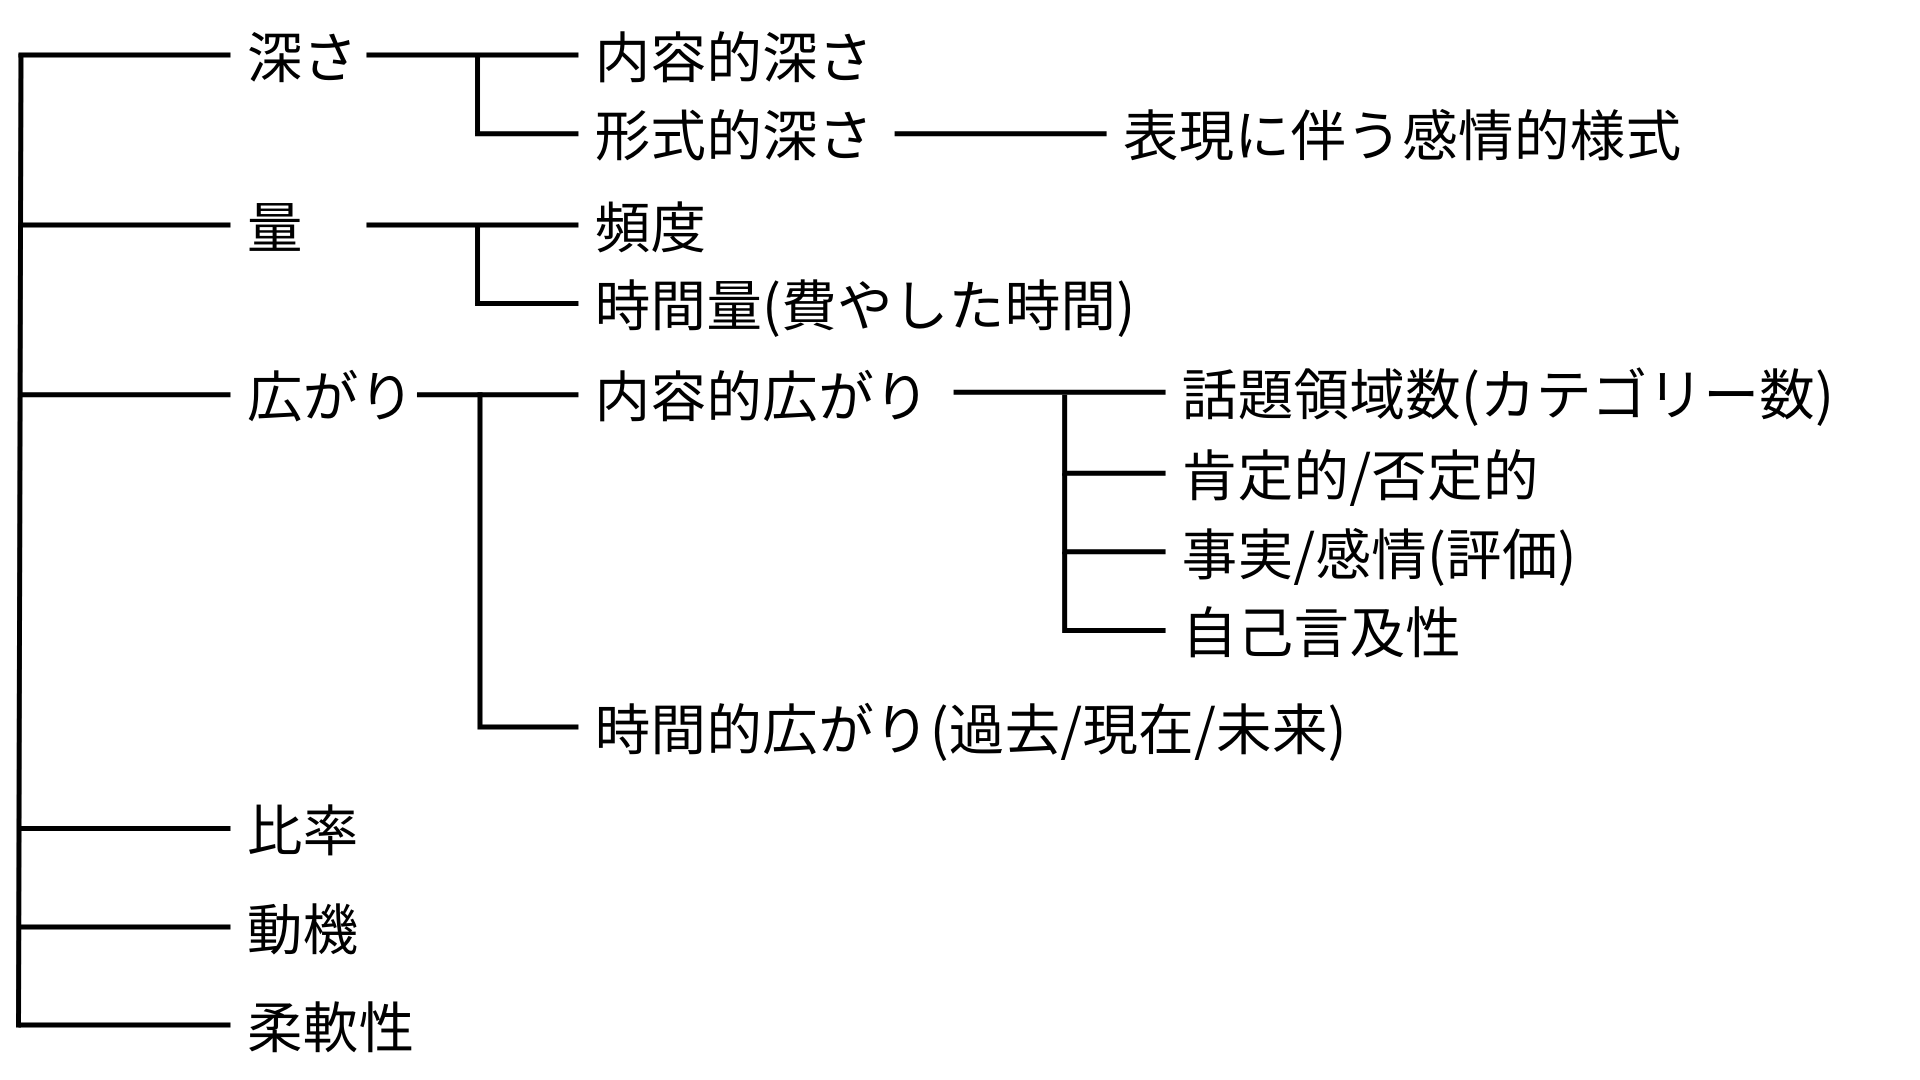
\includegraphics[width=0.75\linewidth]{image/自己開示の次元.png}
    \caption{自己開示の次元}
    \label{fig:自己開示の次元}
\end{figure}

% ＜各次元の説明（全て榎本を参考に）＞
深さの次元は，内容的深さと形式的深さに分類される．内容的深さは開示される情報の本質的な深さを表し，表層的な事実から内面的な感情まで段階的に変化する．形式的深さは表現に伴う感情的様式を示し，感情表現の強さや直接性の程度を反映する．榎本は，この深さの次元が親密な関係性の発展において特に重要な役割を果たすことを指摘している．
量の次元は，自己開示の頻度と費やした時間量で測定される．
広がりの次元は，内容的広がりと時間的広がりから構成される．内容的広がりには話題領域数，肯定性/否定性，事実/感情，自己言及性といった次元が含まれ，自己開示の多様性を表す．時間的広がりは過去・現在・未来にわたる開示の範囲を示し，時間軸における開示内容の分布を反映する．
比率の次元は全体的なコミュニケーションにおける自己開示の割合を表し，関係性の質を反映する指標となる．
動機の次元は，自己開示を行う理由や目的を示し，関係性の発展や維持における意図的な側面を反映する．
柔軟性の次元は状況や相手に応じて自己開示の程度を調整する能力を表し，社会的スキルの一側面として捉えられる．

% その中で，深さに着目する理由を述べる．
Collinsら\cite{collins_1994}のメタ分析によると．自己開示の量よりも深さが好意形成に大きな効果をもたらすことが示されている．また社会的浸透理論という理論では．関係性は自己開示の深さと広さの段階的な増加を通して発展することが提案されている．これらの知見に基づき，本研究では，親密化の過程における影響が大きいとされる深さに着目する．次項では，この自己開示の深さについて社会的浸透理論を元に詳しく論じる．



\subsection{自己開示の深さ}\label{自己開示の深さ}

自己開示における深さとは，開示される個人的な情報の度合いを指す．Derlega\cite{derlega_1993_self_disclosure}によれば，表面的な事実（趣味や職業など）から，内面的な感情（家族の問題や人生の目標に関する感情など）まで，様々な深さの段階が存在する．

自己開示の深さについて，Altman・Taylor（1973）の見解を榎本は以下のように整理している：
\begin{enumerate}
    \item 特定の状況下の個々の行動の開示より，性格特性のようなより普遍的な傾向の開示のほうが深い
    \item 独自な内容の開示ほど深い
    \item 行動や実際の出来事よりも，動機・感情・空想のような目に見えない側面の開示ほど深い
    \item 自分の弱点にふれる内容の開示ほど深い
    \item 社会的に望ましくない側面の開示ほど深い
    \item 強い感情を伴う開示ほど深い
\end{enumerate}

このような深さの概念を体系的に説明する理論として，社会的浸透理論（Social Penetration Theory）がある．

\subsection*{社会的浸透理論}
社会的浸透理論では，2者間の相互作用が表面的なレベルから親密なレベルへと進展し，人間関係が親密化していく過程を社会的浸透（Social Penetration）という概念で説明している．この理論では，人間関係における自己開示の深まりを玉ねぎの層に喩え，表面的な層から徐々により深い層へと進展していく段階的なプロセスをモデル化している．図\ref{fig:onion-model}に自己開示の段階を表す玉ねぎモデルを示す．

\begin{figure}[H]
    \centering
    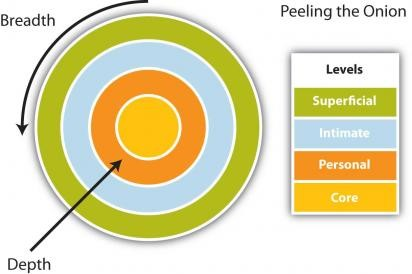
\includegraphics[width=0.75\linewidth]{image/onion-model.png}
    \caption{自己開示の段階を表す玉ねぎモデル}
    \label{fig:onion-model}
\end{figure}

Poseyら\cite{posey_2010}は内側の親密な層が明らかにされる前に，外層の部分が順番に露出し，経験され，剥がされなければならないと述べており，自己開示の深まりには段階的なプロセスが必要であることを指摘している．

また，社会的浸透理論において，自己開示の各層は以下のように整理されている．

\begin{enumerate}
    \item 表層：服装や音楽の好き嫌いなど，比較的浅い情報
    \item 中間層：政治的な見解，社会的な態度
    \item 内層：精神的な価値観，深い恐れ，希望，目標，空想，秘密
    \item 核：その人に関する最もプライベートな情報
\end{enumerate}

本項では，社会的浸透理論に基づき自己開示の深さについて論じた．自己開示は表層的な内容から徐々により深い内容へと段階的に進展していくプロセスを経ることを示し，玉ねぎモデルで4つの層に分けて整理した．自己開示の深さには，様々な状況要因が影響を与えることが知られている．次項では，自己開示の促進に関わる状況要因について説明する．



\subsection{自己開示に影響する状況要因}\label{状況要因}

自己開示は状況とも密接な関係がある．榎本は，自己開示に影響を与える状況要因として，相手の性別，人種，魅力度（外見など），両者の地位関係，部屋のつくりや装飾，視線，自意識の喚起度，生理的条件（飲酒等）など，多くの要因を指摘している．しかし，最大の要因は相手の自己開示の程度，すなわち自己開示の相互性であると述べており，この要因は個人差を打ち消してしまうほど強い影響力を持つことが，多くの研究により実証されている．


\subsection*{自己開示の相互性}\label{自己開示の相互性}

榎本は自己開示の相互性とは，相手の開示レベルに合わせて自分も開示しようとする傾向であると述べる．相手が浅い自己開示しかしない場合，こちらも浅い自己開示しか行わず，相手が深い自己開示をした場合には，こちらも深い自己開示をするというものである．深田\cite{深田_2000}は，自己開示は開示相手にとって報酬的な意味を持ち，お返しの自己開示を促進することにより，自己開示の相互性が次第に高まり，その結果2者関係が発展すると述べている．
榎本は，自己開示の相互性の時系列的変化についても言及している．表層的な自己開示の相互性については，関係の初期に最も頻繁に表れ，次第に減少していく．一方，深い自己開示の相互性は，関係の初期にはほとんど見られないがしだいに増してゆき，中盤でピークを迎えやがて減少していくという．

% 相互性の崩壊（対象でない関係段階）について
% ただし，この相互性は必ずしも成り立つわけではない．榎本によれば，初対面の関係や非常に親密な関係では，この相互性は崩壊する傾向にあるという．初対面の状況では，自己開示が一定のレベルを超えると，お互いの現在の関係から予期される水準を大きく上回り，開示者に対する不信感が生じる．一方，非常に親密な関係では，既に強固な信頼関係が成立しているため，必ずしも自己開示の返報を必要しないという．

% 総論
上記の通り自己開示の相互性の研究より，相手が自己開示をした際に，最も抵抗なく自己開示をすることができるということが示唆された．自己開示は単一方向的なものではなく，開示者と被開示者の間での相互作用だと考えられる．具体的には，Aの自己開示に対してBが受容をし，その後Bが同程度の自己開示を行うという循環的なプロセスが存在する．このプロセスにおいて，被開示者の受容が重要な役割を果たすことから，次節では自己開示の受容について詳しく検討する．